
\documentclass[12pt]{article}

% Layout.
\usepackage[top=1in, bottom=0.75in, left=1in, right=1in, headheight=1in, headsep=6pt]{geometry}

% Fonts.
\usepackage{mathptmx}
\usepackage[scaled=0.86]{helvet}
\renewcommand{\emph}[1]{\textsf{\textbf{#1}}}

% TiKZ.
\usepackage{tikz, pgfplots}
\usetikzlibrary{calc}
\pgfplotsset{compat = newest}
 
\pgfplotsset{my style/.append style={axis x line=middle, axis y line=
middle, xlabel={$x$}, ylabel={$y$}, axis equal }}

% Misc packages.
\usepackage{amsmath,amssymb,latexsym}
\usepackage{graphicx}
\usepackage{array}
\usepackage{xcolor}
\usepackage{multicol}

% Commands to set various header/footer components.
\makeatletter
\def\doctitle#1{\gdef\@doctitle{#1}}
\doctitle{Use {\tt\textbackslash doctitle\{MY LABEL\}}.}
\def\docdate#1{\gdef\@docdate{#1}}
\docdate{Use {\tt\textbackslash docdate\{MY DATE\}}.}
\def\doccourse#1{\gdef\@doccourse{#1}}
\let\@doccourse\@empty
\def\docscoring#1{\gdef\@docscoring{#1}}
\let\@docscoring\@empty
\def\docversion#1{\gdef\@docversion{#1}}
\let\@docversion\@empty
\makeatother

% Headers and footers layout.
\makeatletter
\usepackage{fancyhdr}
\pagestyle{fancy}
\fancyhf{} % Clears all headers/footers.
\lhead{\baselineskip 30pt
%\emph{\@doctitle\hfill\@docdate}
\emph{\@docdate\hfill\@doctitle}
\ifnum \value{page} > 1\relax\else\\
\emph{Name: \rule{3.5in}{1pt}\hfill \@docscoring}\fi}
\rfoot{\emph{\@docversion}}
\lfoot{\emph{\@doccourse}}
\cfoot{\emph{\thepage}}
\renewcommand{\headrulewidth}{0pt}%
\makeatother

% Paragraph spacing
\parindent 0pt
\parskip 6pt plus 1pt

% A problem is a section-like command. Use \problem{5} to
% start a problem worth 5 points.
\newcounter{probcount}
\newcounter{subprobcount}
\setcounter{probcount}{0}
\newcommand{\problem}[1]{%
\par
\addvspace{4pt}%
\setcounter{subprobcount}{0}%
\stepcounter{probcount}%
\makebox[0pt][r]{\emph{\arabic{probcount}.}\hskip1ex}\emph{[#1 points]}\hskip1ex}
\newcommand{\thesubproblem}{\emph{\alph{subprobcount}.}}

% Subproblems are an enumerate-like environment with a consistent
% numbering scheme. 
% Use \begin{subproblems}\item...\item...\end{subproblems}
\newenvironment{subproblems}{%
\begin{enumerate}%
\setcounter{enumi}{\value{subprobcount}}%
\renewcommand{\theenumi}{\emph{\alph{enumi}}}}%
{\setcounter{subprobcount}{\value{enumi}}\end{enumerate}}

% Blanks for answers in normal and math mode.
\newcommand{\blank}[1]{\rule{#1}{0.75pt}}
\newcommand{\mblank}[1]{\underline{\hspace{#1}}}
\def\emptybox(#1,#2){\framebox{\parbox[c][#2]{#1}{\rule{0pt}{0pt}}}}

% Misc.
\renewcommand{\d}{\displaystyle}
\newcommand{\ds}{\displaystyle}
\def\bc{\begin{center}}
\def\ec{\end{center}}
\def\be{\begin{enumerate}}
\def\ee{\end{enumerate}}


\doctitle{Math 251: Quiz 4}
\docdate{Sept 16, 2021}
\doccourse{UAF Calculus I}
\docversion{v-1}
\docscoring{\blank{0.8in} / 25}
\begin{document}
%\textbf{Please circle your instructor's name:} \hfill Leah Berman  \hfill   Jill Faudree\\

There are 25 points possible on this quiz. No aids (book, calculator, etc.)
are permitted.  {\emph{Show all work for full credit.}}

\problem{4} The function $C(y)= \frac{18(1 +y)}{2y+5}$ models a herd of caribou where $C$ is the number of caribou in hundreds and $y$ is measured in years starting in the year 2000. 
 
%\textcolor{red}{Like 2.3 \#97,98,103,125 respectively}

\begin{subproblems}
\item Observe that $C(10)=7.92.$ Interpret this fact in the context of the problem. To earn full credit your answer should be a complete sentence and must include units.
\vfill

\item It can be shown that $C'(10)=0.0864.$ Interpret this fact in the context of the problem. To earn full credit your answer should be a complete sentence and must include units.
\vfill

\end{subproblems}

\problem{4} The function $y=H(x)$ is graphed below. Sketch the graph of $H'(x)$ on the same set of axes. 

\begin{center}
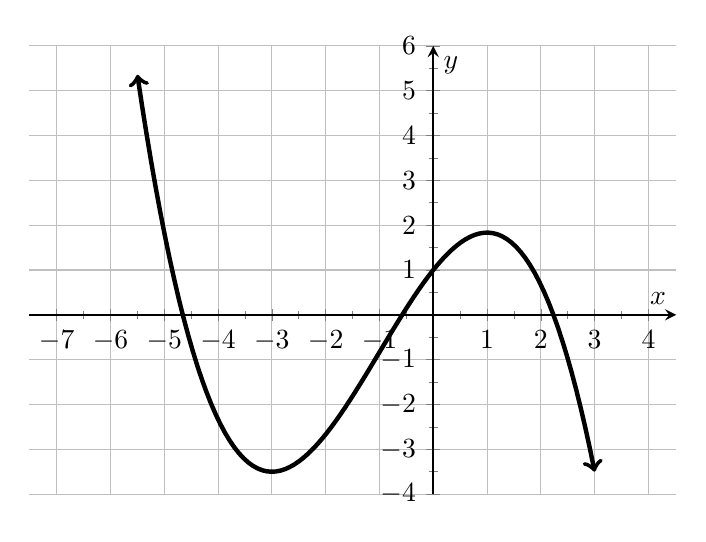
\begin{tikzpicture}
%cubic
\begin{axis}[xscale=1.2, thick, my style, xtick={-7,-6,-5,...,3,4}, ytick={-10,-9,...,11},xmin=-6, xmax=3, ymin=-4, ymax=6, minor y tick num=1, minor x tick num=1, 
mark size=3.0pt, grid = major]
\addplot[ultra thick, <->,domain=-5.5:3, samples=100]{((3*x)/2) - x^2/2 - x^3/6+1};
\end{axis}
\end{tikzpicture}\end{center}
\newpage
\problem{9} Find the derivative of $f(x)=3\sqrt{x}$ \textbf{using the limit definition of the derivative.} No credit will be given for an answer that uses the power rule.
\vspace{4in}
\problem{8} For each function below, find its derivative. You may use any method you like. You do not have to simplify your answer.
\begin{subproblems}
\item $f(x)=\frac{x^3+x-\pi^2}{3}$
\vfill
\item $g(x)= x \left(\frac{1}{x^2}+\frac{1}{x} \right)$
\vfill
%\item $h(x)=\frac{8x}{3-x}$ \textcolor{red}{I am remembering your observation that your students will be seeing the quotient rule for the first time on Wednesday and that testing it on Thursday may be too fast. My  instinct is to leave this problem off...}
\end{subproblems}

\end{document}